\section{Consuntivo}
In questa sezione verrà trattato il rendiconto dei risultati dei costi sostenuti in ogni periodo di attività. Per migliorare la leggibilità dei dati verranno riportate, per ogni periodo, delle tabelle riportanti i vari ruoli, le ore preventivate, quelle consuntivate e i relativi costi mettendo in evidenza se il bilancio del periodo è in \textbf{positivo}, in \textbf{negativo} o in \textbf{pari}. 
\subsection{Analisi}
Si è deciso di riportare il consuntivo di questo periodo, nonostante il costo prodotto in questo lasso di tempo non venga posto a carico del proponente, per utilità interna al gruppo; infatti grazie ad essa si è potuto constatare come le misure messe in atto per contrastare l' inesperienza del gruppo in materia di pianificazione e di controllo dei costi siano state efficaci ed abbiano permesso di concludere il periodo di Analisi in \textbf{positivo} di 70\euro .
\begin{center}
\begin{tabular}{| l | c | c | c | c |}
\hline
\multicolumn{1}{| c |}{Ruoli} & \multicolumn{2}{c}{Preventivo} & \multicolumn{2}{ c|}{Consuntivo}\\
\cline{2-5}
& Ore & Costo (\euro) & Ore & Costo(\euro) \\
\hline
Responsabile & 30 & 900 & 28 & 840 \\
Amministratore & 34 & 680 & 32 & 640\\
Analista & 68 & 1700 & 68 & 1700 \\
Progettista & 0 & 0 & 0 & 0 \\
Verificatore & 26 & 390 & 28 & 420 \\
Programmatore & 0 & 0 & 0 & 0 \\
\hline
\textbf{Totale} & 158 & 3670 & 156 & 3600 \\
\hline
\end{tabular}
\\
Tabella 13: Tabella di confronto tra preventivo e consuntivo per il periodo di AN.
\end{center}
Dalla tabella 13 si nota come i ruoli di \textit{Responsabile} e \textit{Amministratore} siano stati coinvolti in modo minore di quanto pianificato, mentre c'è stata necessità di una maggiore attività di verifica.
\subsection{Progettazione Architetturale}
Qui di seguito verrà riportata la tabella del consuntivo riguardante il periodo di progettazione architetturale.
\begin{center}
\begin{tabular}{| l | c | c | c | c |}
\hline
\multicolumn{1}{| c |}{Ruoli} & \multicolumn{2}{c}{Preventivo} & \multicolumn{2}{ c|}{Consuntivo}\\
\cline{2-5}
& Ore & Costo (\euro) & Ore & Costo(\euro) \\
\hline
Responsabile & 38 & 1140 & 21 & 630 \\
Amministratore & 6 & 120 & 29 & 580 \\
Analista & 48 & 67 & 20 & 500 \\
Progettista & 67 & 1474 & 91 & 2002 \\
Verificatore & 22 & 330 & 26 & 390 \\
Programmatore & 0 & 0 & 0 & 0 \\
\hline
\textbf{Totale} & 181 & 4264 & 187 & 4102 \\
\hline
\end{tabular}
\\
Tabella 14: Tabella di confronto tra preventivo e consuntivo per il periodo di PA.
\end{center}
Dalla tabella 14 si nota come i ruoli di \textit{Responsabile} e \textit{Analista}, quest'ultimo in particolare, siano stati coinvolti in modo minore di quanto pianificato, per quanto riguarda l' analista ciò è dato dal fatto che si era immaginato che i requisiti e l'analisi in generale avessero bisogno di una mole maggiore di correzioni.\\
Le ore di \textit{Progettista} sono aumentate rispetto al preventivo, questo perché il team si è ritrovato durante la progettazione dell'architettura ad effettuare dei cambiamenti dati dall'inesperienza del team in materia di progettazione.\\
Al termine di questo periodo il team \gruppo è riuscito a concludere in positivo di  162\euro .
\subsection{Progettazione di Dettaglio e Codifica}
Qui di seguito viene riportata la tabella del consuntivo riguardante il periodo di progettazione di dettaglio e codifica.
\begin{center}
\begin{tabular}{| l | c | c | c | c |}
\hline
\multicolumn{1}{| c |}{Ruoli} & \multicolumn{2}{c}{Preventivo} & \multicolumn{2}{ c|}{Consuntivo}\\
\cline{2-5}
& Ore & Costo (\euro) & Ore & Costo(\euro) \\
\hline
Responsabile & 35 & 1050 & 6 & 180 \\
Amministratore & 8 & 160 & 6 & 120 \\
Analista & 5 & 125 & 15 & 375 \\
Progettista & 81 & 1781 & 167 & 3674 \\
Verificatore & 93 & 1395 & 40 & 600 \\
Programmatore & 64 & 960 & 48 & 720 \\
\hline
\textbf{Totale} & 286 & 5472 & 282 & 5669 \\
\hline
\end{tabular}
\\
Tabella 14: Tabella di confronto tra preventivo e consuntivo per il periodo di PDC.
\end{center}
Al termine di questo periodo il team \emph{Sirius} ha speso di più di quanto pianificato andando in negativo di 197\euro  ciò è dato dai fattori che verranno trattati qui di seguito. 
Innanzitutto dalla tabella si nota subito che il ruolo del \emph{progettista} è stato il più richiesto dell' intero periodo e il suo numero di ore effettive del periodo si distacca largamente da quanto pianificato; questo perchè è stato  necessario modificare la specifica tecnica in vari punti in quanto non erano stati considerati molti fattori legati all' utilizzo dei \textit{framework} \emph{Spring} e \emph{Backbone}, infatti a causa di tutto ciò è stato  necessario apportare grandi modifiche ai presenter lato client e server, nate anche dalle considerazioni riportate nella correzione del periodo di progettazione architetturale.
Il ruolo di \emph{responsabile} non è stato coinvolto come quanto pianificato, infatti la sua necessità è stata sovrastimata durante la pianificazione delle attività in quanto si pensava ci sarebbe stato maggior bisogno del suo intervento.
Anche il ruolo di \emph{verificatore} è stato poco utilizzato, ma questo non è dovuto a un errore di sovrastima, infatti c'è ancora una grande necessità di eseguire attività di verifica, ma in quanto è stato necessario rivedere l' architettura del sistema in modo quanto più ottimale possibile, si è deciso di utilizzare maggiormente le risorse nella stesura dei documenti di \DefinizioneDiProdotto  e di \SpecificaTecnica  sperando di ridurre così nel periodo di Validazione la necessità di \emph{progettisti}, andando a utilizzare le risorse risparmiate in \emph{verificatori}.
\subsubsection{Conclusioni}
Il gruppo \emph{Sirius} nei precedenti periodi ha risparmiato 192\euro , aggiungendo a tale cifra i 197\euro di negativo di questo periodo si ottiene che il budget è in negativo di 5\euro , anche se tale cifra non è elevata, è comunque un indice negativo e i soldi risparmiati in precedenza non possono essere più usati per attività di verifica e validazione ulteriori sul prodotto; ad ogni modo avendo realizzato un' architettura di dettaglio quanto più ottimale possibile, non dovrebbe essere necessario nel prossimo periodo apportarci grandi modifiche, quindi sarà possibile incentrare le risorse del team in attività di verifica e validazione andando così a migliorare la qualità del software realizzato.
\subsection{Validazione}
Qui di seguito viene riportata la tabella del consuntivo riguardante il periodo di validazione.
\begin{center}
\begin{tabular}{| l | c | c | c | c |}
\hline
\multicolumn{1}{| c |}{Ruoli} & \multicolumn{2}{c}{Preventivo} & \multicolumn{2}{ c|}{Consuntivo}\\
\cline{2-5}
& Ore & Costo (\euro) & Ore & Costo(\euro) \\
\hline
Responsabile & 33 & 990 & 2 & 60 \\
Amministratore & 20 & 400 & 2 & 40 \\
Analista & 0 & 0 & 0 & 0 \\
Progettista & 24 & 528 & 8 & 176 \\
Verificatore & 77 & 1155 & 125 & 1875 \\
Programmatore & 15 & 225 & 24 & 360 \\
\hline
\textbf{Totale} & 169 & 3298 & 161 & 2511 \\
\hline
\end{tabular}
\\
Tabella 15: Tabella di confronto tra preventivo e consuntivo per il periodo di VV.
\end{center}
Come si può subito notare le ore, ma in particolare il costo di questo periodo, si discostano molto da quanto preventivato e andremo ora a esaminare i ruoli più rilevanti e il loro utilizzo durante questo periodo.
\subsubsection{Verificatore}
Certamente il ruolo più attivo dell' intero periodo, infatti è stato necessario eseguire una grande quantità di test sia nella parte server, sia nella parte client dopo aver modificato buona parte dell' architettura nel periodo precedente. Il condensarsi di tutte queste ore in questo periodo è dato dal fatto che il gruppo non era stato in grado di dedicare abbastanza ore ai test nel periodo precedente in quanto aveva dovuto concentrarsi sulla stesura di una architettura solida e a sviluppare una \textit{demo} funzionante. Certamente tutto si sarebbe potuto evitare realizzando una architettura sana in principio.
\subsubsection{Programmatore}
La differenza di ore non è molta, ciononostante sono state necessarie ore extra rispetto a quanto preventivato, questo è stato dato dal fatto che dopo l' incontro con Gregorio Piccoli, è stato necessario apportare piccole modifiche all ' interfaccia grafica e anche al server. Certamente se un incontro con il proponente fosse stato fissato prima si sarebbe potuto ottenere un \textit{feedback} che avrebbe permesso al gruppo di risparmiare queste ore.
\subsubsection{Progettista}
L' architettura sviluppata nel precedente periodo è stata sviluppata abbastanza bene e a parte errori nella documentazione, non è stato necessario modificare quasi nulla nell' architettura. Certamente le ore risparmiate in questo periodo sono un magro compenso rispetto all' enorme quantità di ore in eccesso nel precedente periodo.
\subsection{Totale}
Viene riportato di seguito il consuntivo dell' intero sviluppo del progetto.\\
Qui di seguito viene riportata la tabella che riporta le ore preventivate e effettive al termine dello sviluppo del progetto, senza prendere in considerazione il periodo di Analisi.
\begin{center}
\begin{tabular}{| l | c | c | c | c |}
\hline
\multicolumn{1}{| c |}{Ruoli} & \multicolumn{2}{c}{Preventivo} & \multicolumn{2}{ c|}{Consuntivo}\\
\cline{2-5}
& Ore & Costo (\euro) & Ore & Costo(\euro) \\
\hline
Responsabile & 106 & 3180 & 29 & 870 \\
Amministratore & 34 & 680 & 37 & 740 \\
Analista & 53 & 1325 & 35 & 875 \\
Progettista & 172 & 3784 & 266 & 5852 \\
Verificatore & 192 & 2880 & 191 & 2865 \\
Programmatore & 79 & 1185 & 72 & 1080 \\
\hline
\textbf{Totale} & 636 & 13034 & 630 & 12282 \\
\hline
\end{tabular}
\\
Tabella 16: Tabella di confronto tra preventivo e consuntivo per l' intero periodo di sviluppo(analisi esclusa).
\end{center}
\begin{center}
\begin{tabular}{| l | c | c | c | c | c | c | c |}
\hline
Membro & Re & Am & An & Pt & Ve & Pr & ore totali \\
\hline
Botter Marco & 4 & 4 & 4 & 52 & 29 & 12 & 105 \\

Giachin Vanni & 8 & 8 & 9 & 48 & 19 & 13 & 105 \\

Marcomin Gabriele & 6 & 7 & 2 & 53 & 24 & 13 & 105 \\

Quaglio Davide & 5 & 9 & 9 & 45 & 25 & 12 & 105 \\

Santangelo Davide & 2 & 7 & 3 & 33 & 50 & 10 & 105 \\

Seresin Davide & 4 & 2 & 8 & 35 & 44 & 12 & 105 \\
\hline
\end{tabular}
\\
Tabella 17: Ore per membro,senza periodo di analisi.
\end{center}
Il seguente grafico riporta le ore effettivamente impiegate da ciascun componente per lo sviluppo del progetto senza prendere in considerazione il periodo di analisi
\begin{figure}[H] \centering 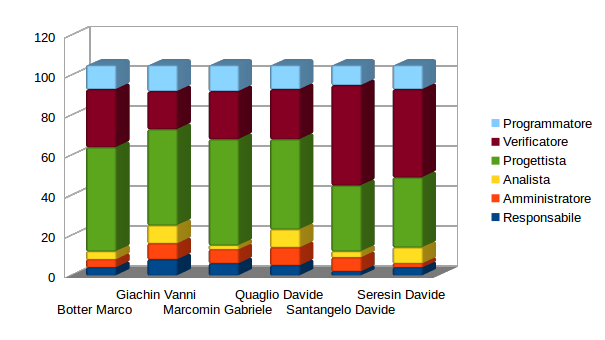
\includegraphics[width=%
\textwidth]
{../modello/img/totruoli.png} \caption{ore impiegate da ciascun componente}
\end{figure}
\subsubsection{Conclusioni}
Come si può notare da quanto riportato sopra, sono state impiegate \textbf{105} ore per ciascun componente determinando un costo totale di \textbf{12282\euro} . Rispetto a quanto preventivato il gruppo è riuscito a risparmiare 752\euro , ciononostante, dati i problemi avuti durante il periodo di progettazione di dettaglio e codifica che poi hanno avuto effetto anche nell' ultimo periodo, andando a variare in modo rilevante le ore e le attività pianificate, sarebbe stato possibile ottenere un ben più largo guadagno, che con il senno di poi si sarebbe facilmente ottenuto con una pianificazione dalla grana più fine, e ponendo una particolare attenzione alle singole esigenze dei singoli componenti del gruppo.